% Diagramas reproducibles, en blanco y negro. Compilar con pdflatex.
% Alcance de «actual»: lab019_first_ekf_full_batch.source.ipynb,
% funciones core_batch, gate, history y rhs_batch (sólo el modelo dinámico).
% Prima el código de ese notebook sobre documentos históricos: alpha=44.01/46.07,
% activación por azúcar predicho, sin término respiratorio independiente.
% Zenteno: context/modeling/Zenteno_2010.pdf, sección 2.7, ecuaciones 14--16.
% Adaptación a un reactor homogéneo con volumen constante y T medida;
% se conserva nuestro núcleo biológico, no los compartimentos térmicos del paper.
% Las ecuaciones de Zenteno son una referencia propuesta, no código ejecutado.
\documentclass[10pt]{article}
\usepackage[a3paper,landscape,margin=12mm]{geometry}
\usepackage[utf8]{inputenc}
\usepackage[T1]{fontenc}
\usepackage{lmodern,amsmath,amssymb,tikz}
\usetikzlibrary{arrows.meta,calc}
\usepackage[hidelinks]{hyperref}
\hypersetup{pdftitle={Modelo actual y adaptación a Zenteno: diagramas de bloques},
  pdfsubject={Núcleo biológico, estados dinámicos, producción y liberación de CO2}}
\pagestyle{empty}
\setlength{\parindent}{0pt}
\newcommand{\clip}{\operatorname{clip}}
\newcommand{\pos}[1]{\left[#1\right]_+}
\newcommand{\bb}{\mathbf b}
\newcommand{\block}[7]{%
  \node[draw,rectangle,anchor=north west,align=center,inner sep=2mm,
    minimum width=#4cm,minimum height=#5cm,text width=\dimexpr #4cm-4mm\relax]
    (#1) at (#2,#3) {\textbf{#6}\\[4pt]#7};}
\tikzset{flow/.style={-{Latex[length=2mm,width=1.3mm]},line width=.6pt,
    preaction={draw=white,line width=2.8pt,arrows=-}},
  signal/.style={font=\small,fill=white,inner sep=1.2pt,align=center}}

\begin{document}
\begin{center}
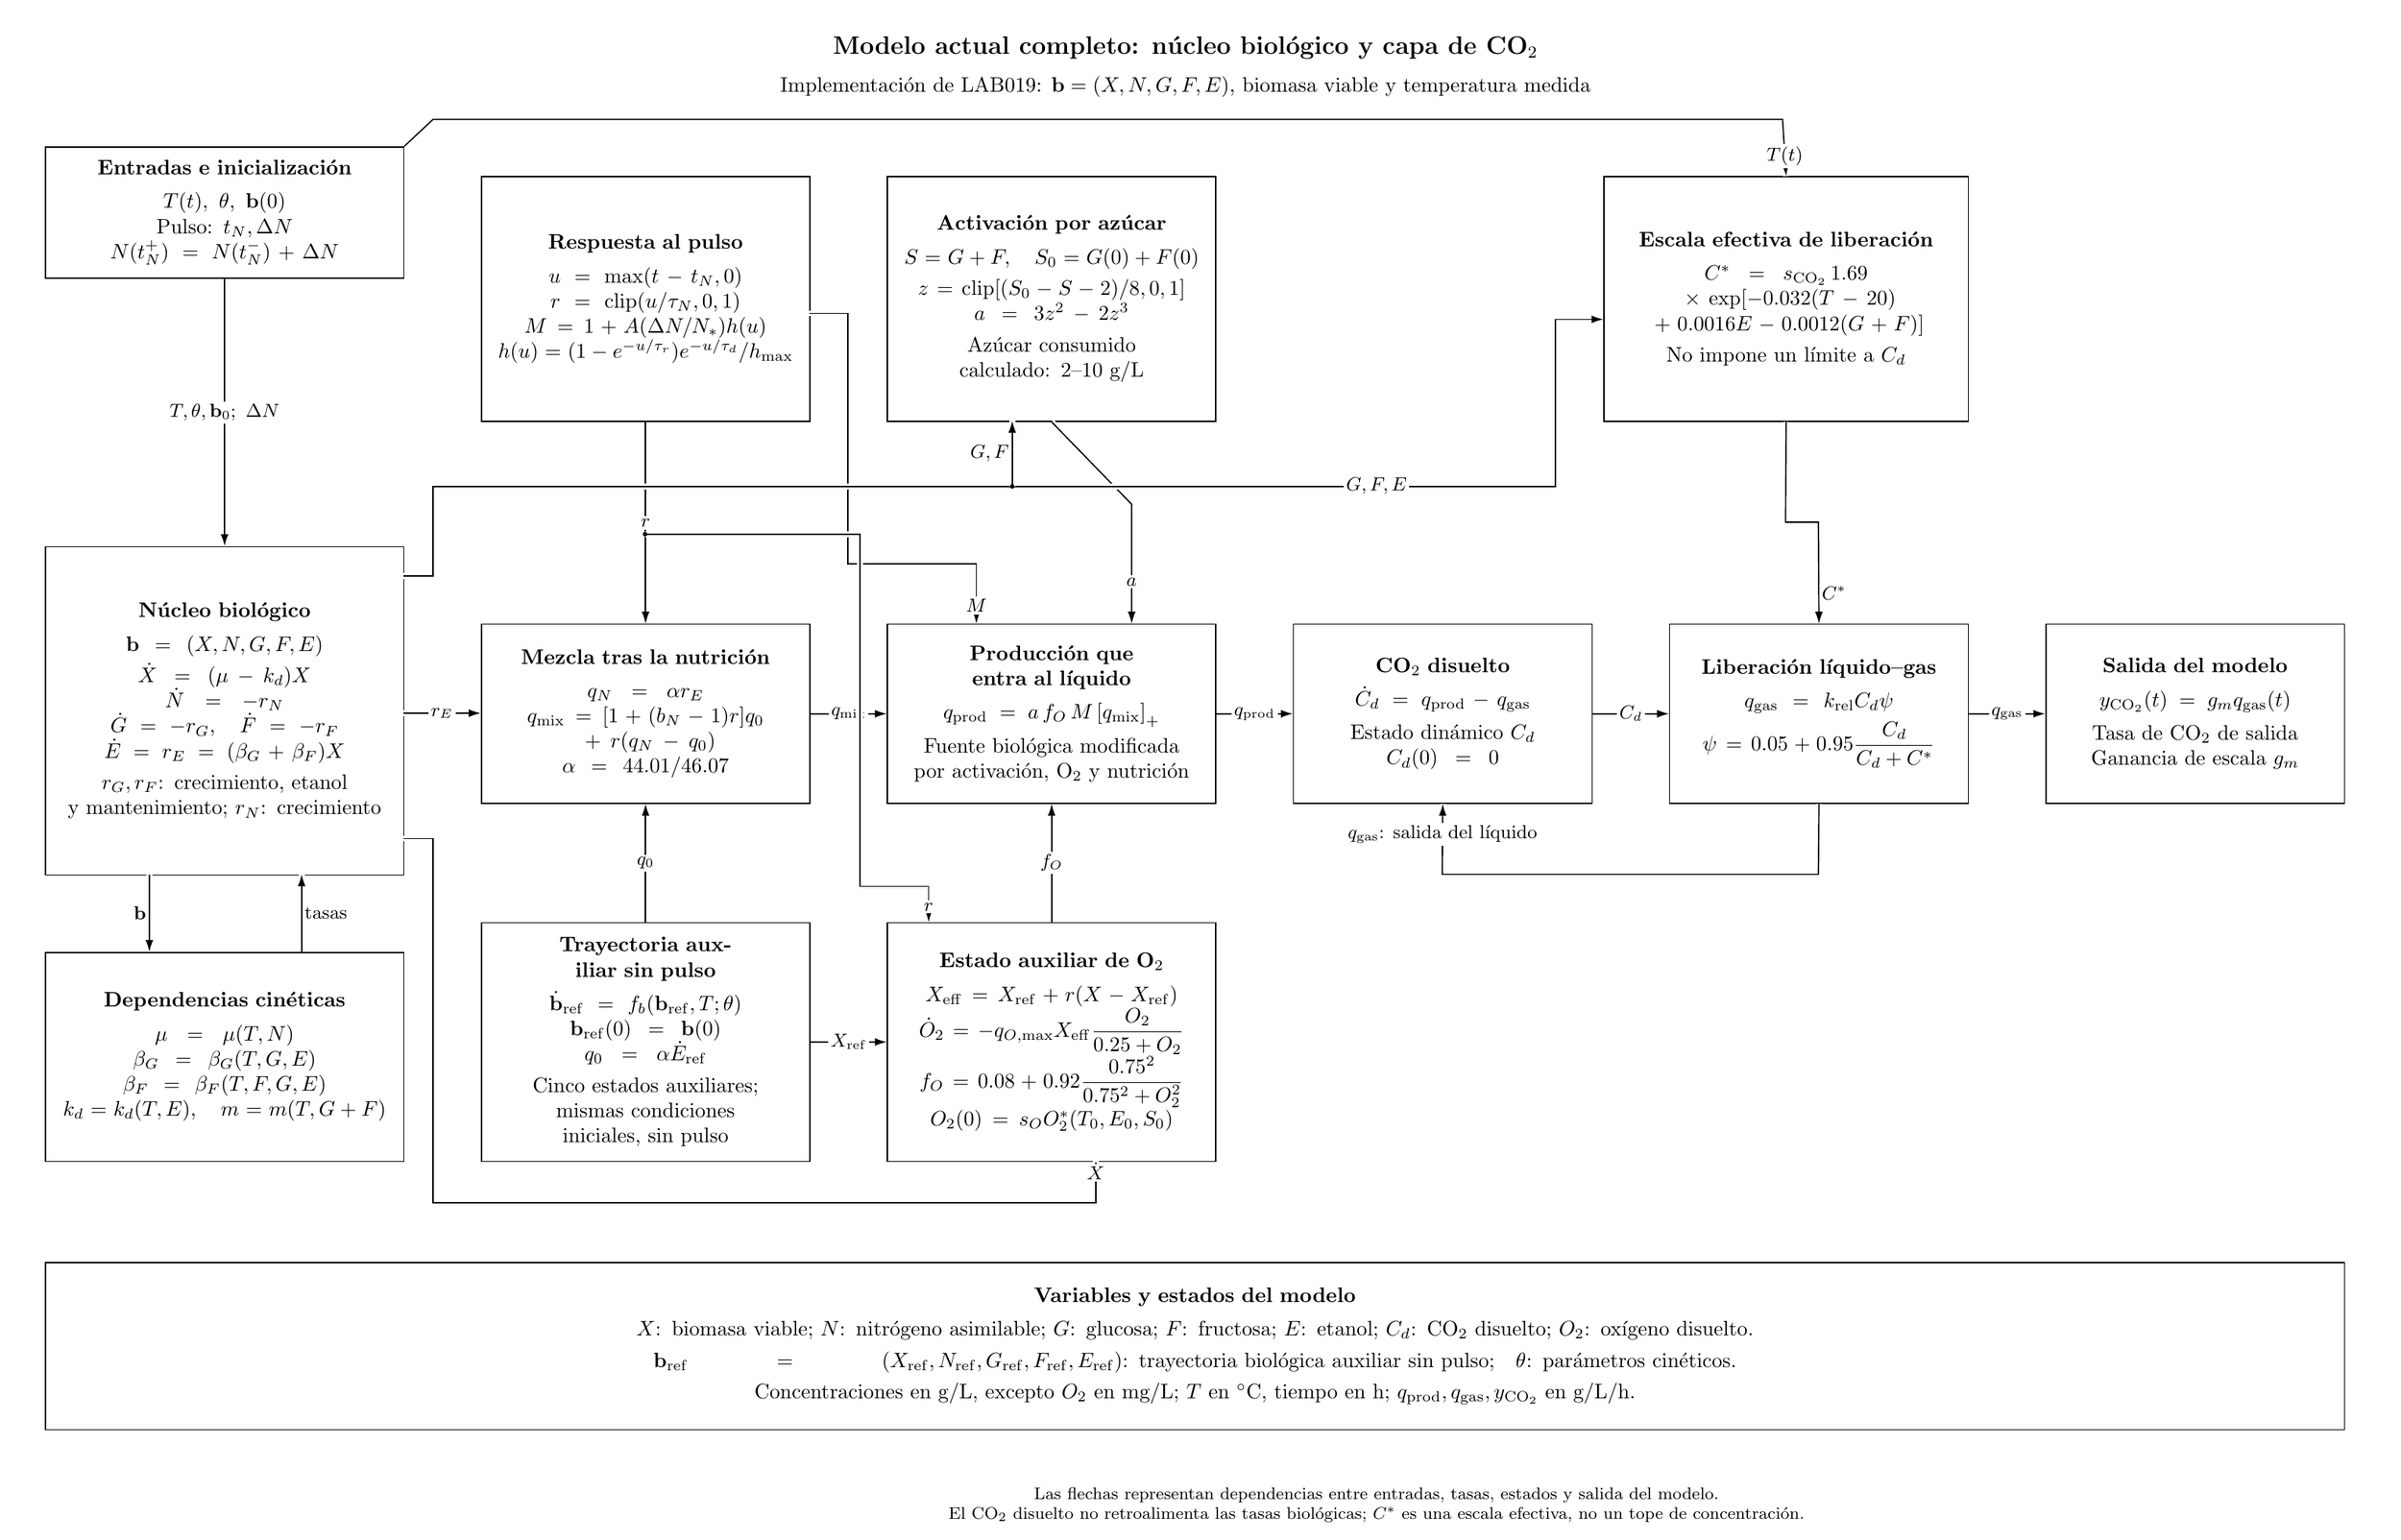
\begin{tikzpicture}[x=1cm,y=1cm,font=\normalsize,line width=.55pt]
\useasboundingbox (0,0) rectangle (39.5,25.1);
\node[font=\large\bfseries] at (19.5,24.65)
  {Modelo actual completo: núcleo biológico y capa de CO\(_2\)};
\node at (19.5,24.0)
  {Implementación de LAB019: \(\bb=(X,N,G,F,E)\), biomasa viable y temperatura medida};

\block{inputs}{0.4}{23.0}{6.0}{2.2}{Entradas e inicialización}{%
  \(T(t),\ \theta,\ \bb(0)\)\\
  Pulso: \(t_N,\Delta N\)\\
  \(N(t_N^+)=N(t_N^-)+\Delta N\)}
\block{bio}{0.4}{16.3}{6.0}{5.5}{Núcleo biológico}{%
  \(\bb=(X,N,G,F,E)\)\\[3pt]
  \(\dot X=(\mu-k_d)X\)\\
  \(\dot N=-r_N\)\\
  \(\dot G=-r_G,\quad\dot F=-r_F\)\\
  \(\dot E=r_E=(\beta_G+\beta_F)X\)\\[3pt]
  \(r_G,r_F\): crecimiento, etanol\\y mantenimiento; \(r_N\): crecimiento}
\block{rates}{0.4}{9.5}{6.0}{3.5}{Dependencias cinéticas}{%
  \(\mu=\mu(T,N)\)\\
  \(\beta_G=\beta_G(T,G,E)\)\\
  \(\beta_F=\beta_F(T,F,G,E)\)\\
  \(k_d=k_d(T,E),\quad m=m(T,G+F)\)}
\block{nutrition}{7.7}{22.5}{5.5}{4.1}{Respuesta al pulso}{%
  \(u=\max(t-t_N,0)\)\\
  \(r=\clip(u/\tau_N,0,1)\)\\
  \(M=1+A(\Delta N/N_*)h(u)\)\\
  \(h(u)=(1-e^{-u/\tau_r})e^{-u/\tau_d}/h_{\max}\)}
\block{gate}{14.5}{22.5}{5.5}{4.1}{Activación por azúcar}{%
  \(S=G+F,\quad S_0=G(0)+F(0)\)\\[3pt]
  \(z=\clip[(S_0-S-2)/8,0,1]\)\\
  \(a=3z^2-2z^3\)\\[3pt]
  Azúcar consumido calculado: 2--10 g/L}
\block{mix}{7.7}{15.0}{5.5}{3.0}{Mezcla tras la nutrición}{%
  \(q_N=\alpha r_E\)\\
  \(q_{\mathrm{mix}}=[1+(b_N-1)r]q_0\)\\
  \({}+r(q_N-q_0)\)\\
  \(\alpha=44.01/46.07\)}
\block{ref}{7.7}{10.0}{5.5}{4.0}{Trayectoria auxiliar sin pulso}{%
  \(\dot{\bb}_{\mathrm{ref}}=f_b(\bb_{\mathrm{ref}},T;\theta)\)\\
  \(\bb_{\mathrm{ref}}(0)=\bb(0)\)\\
  \(q_0=\alpha\dot E_{\mathrm{ref}}\)\\[3pt]
  Cinco estados auxiliares;\\mismas condiciones iniciales, sin pulso}
\block{prod}{14.5}{15.0}{5.5}{3.0}{Producción que entra al líquido}{%
  \(q_{\mathrm{prod}}=a\,f_O\,M\pos{q_{\mathrm{mix}}}\)\\[4pt]
  Fuente biológica modificada\\por activación, O\(_2\) y nutrición}
\block{oxygen}{14.5}{10.0}{5.5}{4.0}{Estado auxiliar de O\(_2\)}{%
  \(X_{\mathrm{eff}}=X_{\mathrm{ref}}+r(X-X_{\mathrm{ref}})\)\\
  \(\dot O_2=-q_{O,\max}X_{\mathrm{eff}}\dfrac{O_2}{0.25+O_2}\)\\
  \(f_O=0.08+0.92\dfrac{0.75^2}{0.75^2+O_2^2}\)\\
  \(O_2(0)=s_O O_2^*(T_0,E_0,S_0)\)}
\block{inventory}{21.3}{15.0}{5.0}{3.0}{CO\(_2\) disuelto}{%
  \(\dot C_d=q_{\mathrm{prod}}-q_{\mathrm{gas}}\)\\[4pt]
  Estado dinámico \(C_d\)\\
  \(C_d(0)=0\)}
\block{sat}{26.5}{22.5}{6.1}{4.1}{Escala efectiva de liberación}{%
  \(C^*=s_{\mathrm{CO_2}}\,1.69\)\\
  \({}\times\exp[-0.032(T-20)\)\\
  \({}+0.0016E-0.0012(G+F)]\)\\[3pt]
  No impone un límite a \(C_d\)}
\block{release}{27.6}{15.0}{5.0}{3.0}{Liberación líquido--gas}{%
  \(q_{\mathrm{gas}}=k_{\mathrm{rel}}C_d\psi\)\\[3pt]
  \(\psi=0.05+0.95\dfrac{C_d}{C_d+C^*}\)}
\block{obs}{33.9}{15.0}{5.0}{3.0}{Salida del modelo}{%
  \(y_{\mathrm{CO_2}}(t)=g_mq_{\mathrm{gas}}(t)\)\\[4pt]
  Tasa de CO\(_2\) de salida\\
  Ganancia de escala \(g_m\)}
\block{variables}{0.4}{4.3}{38.5}{2.8}{Variables y estados del modelo}{%
  \(X\): biomasa viable; \(N\): nitrógeno asimilable; \(G\): glucosa; \(F\): fructosa;
  \(E\): etanol; \(C_d\): CO\(_2\) disuelto; \(O_2\): oxígeno disuelto.\\[3pt]
  \(\bb_{\mathrm{ref}}=(X_{\mathrm{ref}},N_{\mathrm{ref}},G_{\mathrm{ref}},F_{\mathrm{ref}},E_{\mathrm{ref}})\):
  trayectoria biológica auxiliar sin pulso;\quad \(\theta\): parámetros cinéticos.\\[3pt]
  Concentraciones en g/L, excepto \(O_2\) en mg/L; \(T\) en \(^{\circ}\mathrm C\), tiempo en h;
  \(q_{\mathrm{prod}},q_{\mathrm{gas}},y_{\mathrm{CO_2}}\) en g/L/h.}

% Rutas: la preacción blanca deja un salto visual en cruces sin unión.
\draw[flow] (inputs.south) -- (bio.north) node[midway,signal] {\(T,\theta,\bb_0;\ \Delta N\)};
\draw[flow] (inputs.north east) -- (6.9,23.45) -- (29.5,23.45) -- (sat.north)
  node[pos=.65,signal] {\(T(t)\)};
\draw[flow] (6.4,13.5) -- (7.7,13.5) node[midway,signal] {\(r_E\)};
\draw[flow] (mix.east) -- (prod.west) node[midway,signal] {\(q_{\mathrm{mix}}\)};
\draw[flow] (prod.east) -- (inventory.west) node[midway,signal] {\(q_{\mathrm{prod}}\)};
\draw[flow] (inventory.east) -- (release.west) node[midway,signal] {\(C_d\)};
\draw[flow] (release.east) -- (obs.west) node[midway,signal] {\(q_{\mathrm{gas}}\)};
\draw[flow] (release.south) -- (30.1,10.8) -- (23.8,10.8) -- (inventory.south)
  node[pos=.57,signal] {\(q_{\mathrm{gas}}\): salida del líquido};
\draw[flow] (ref.north) -- (mix.south) node[midway,signal] {\(q_0\)};
\draw[flow] (nutrition.south) -- (mix.north) node[midway,signal] {\(r\)};
\draw[flow] (13.2,20.2) -- (13.85,20.2) -- (13.85,16.0) -- (16.0,16.0) -- (16.0,15.0)
  node[pos=.7,signal] {\(M\)};
\draw[flow] (10.45,16.5) -- (14.05,16.5) -- (14.05,10.6) -- (15.2,10.6) -- (15.2,10.0)
  node[pos=.58,signal] {\(r\)};
\fill (10.45,16.5) circle (1.1pt);
\draw[flow] (gate.south) -- (18.6,17.0) -- (18.6,15.0) node[pos=.65,signal] {\(a\)};
\draw[flow] (oxygen.north) -- (prod.south) node[midway,signal] {\(f_O\)};
\draw[flow] (ref.east) -- (oxygen.west) node[midway,signal] {\(X_{\mathrm{ref}}\)};
\draw[flow] (6.4,11.4) -- (6.9,11.4) -- (6.9,5.3) -- (18.0,5.3) -- (18.0,6.0)
  node[pos=.71,signal] {\(X\)};
\draw[flow] (6.4,15.8) -- (6.9,15.8) -- (6.9,17.3) -- (25.7,17.3) -- (25.7,20.1) -- (26.5,20.1)
  ;
\node[signal] at (22.7,17.3) {\(G,F,E\)};
\draw[flow] (16.6,17.3) -- (16.6,18.4) node[midway,signal,left] {\(G,F\)};
\fill (16.6,17.3) circle (1.1pt);
\draw[flow] (sat.south) -- (29.55,16.7) -- (30.1,16.7) -- (release.north)
  node[pos=.7,signal,right] {\(C^*\)};
\draw[flow] (2.15,10.8) -- (2.15,9.5) node[midway,signal,left] {\(\bb\)};
\draw[flow] (4.7,9.5) -- (4.7,10.8) node[midway,signal,right] {tasas};
\node[anchor=north,align=center,font=\footnotesize] at (22.7,.65)
  {Las flechas representan dependencias entre entradas, tasas, estados y salida del modelo.\\
   El CO\(_2\) disuelto no retroalimenta las tasas biológicas; \(C^*\) es una escala efectiva, no un tope de concentración.};
\end{tikzpicture}
\end{center}

\newpage
\begin{center}
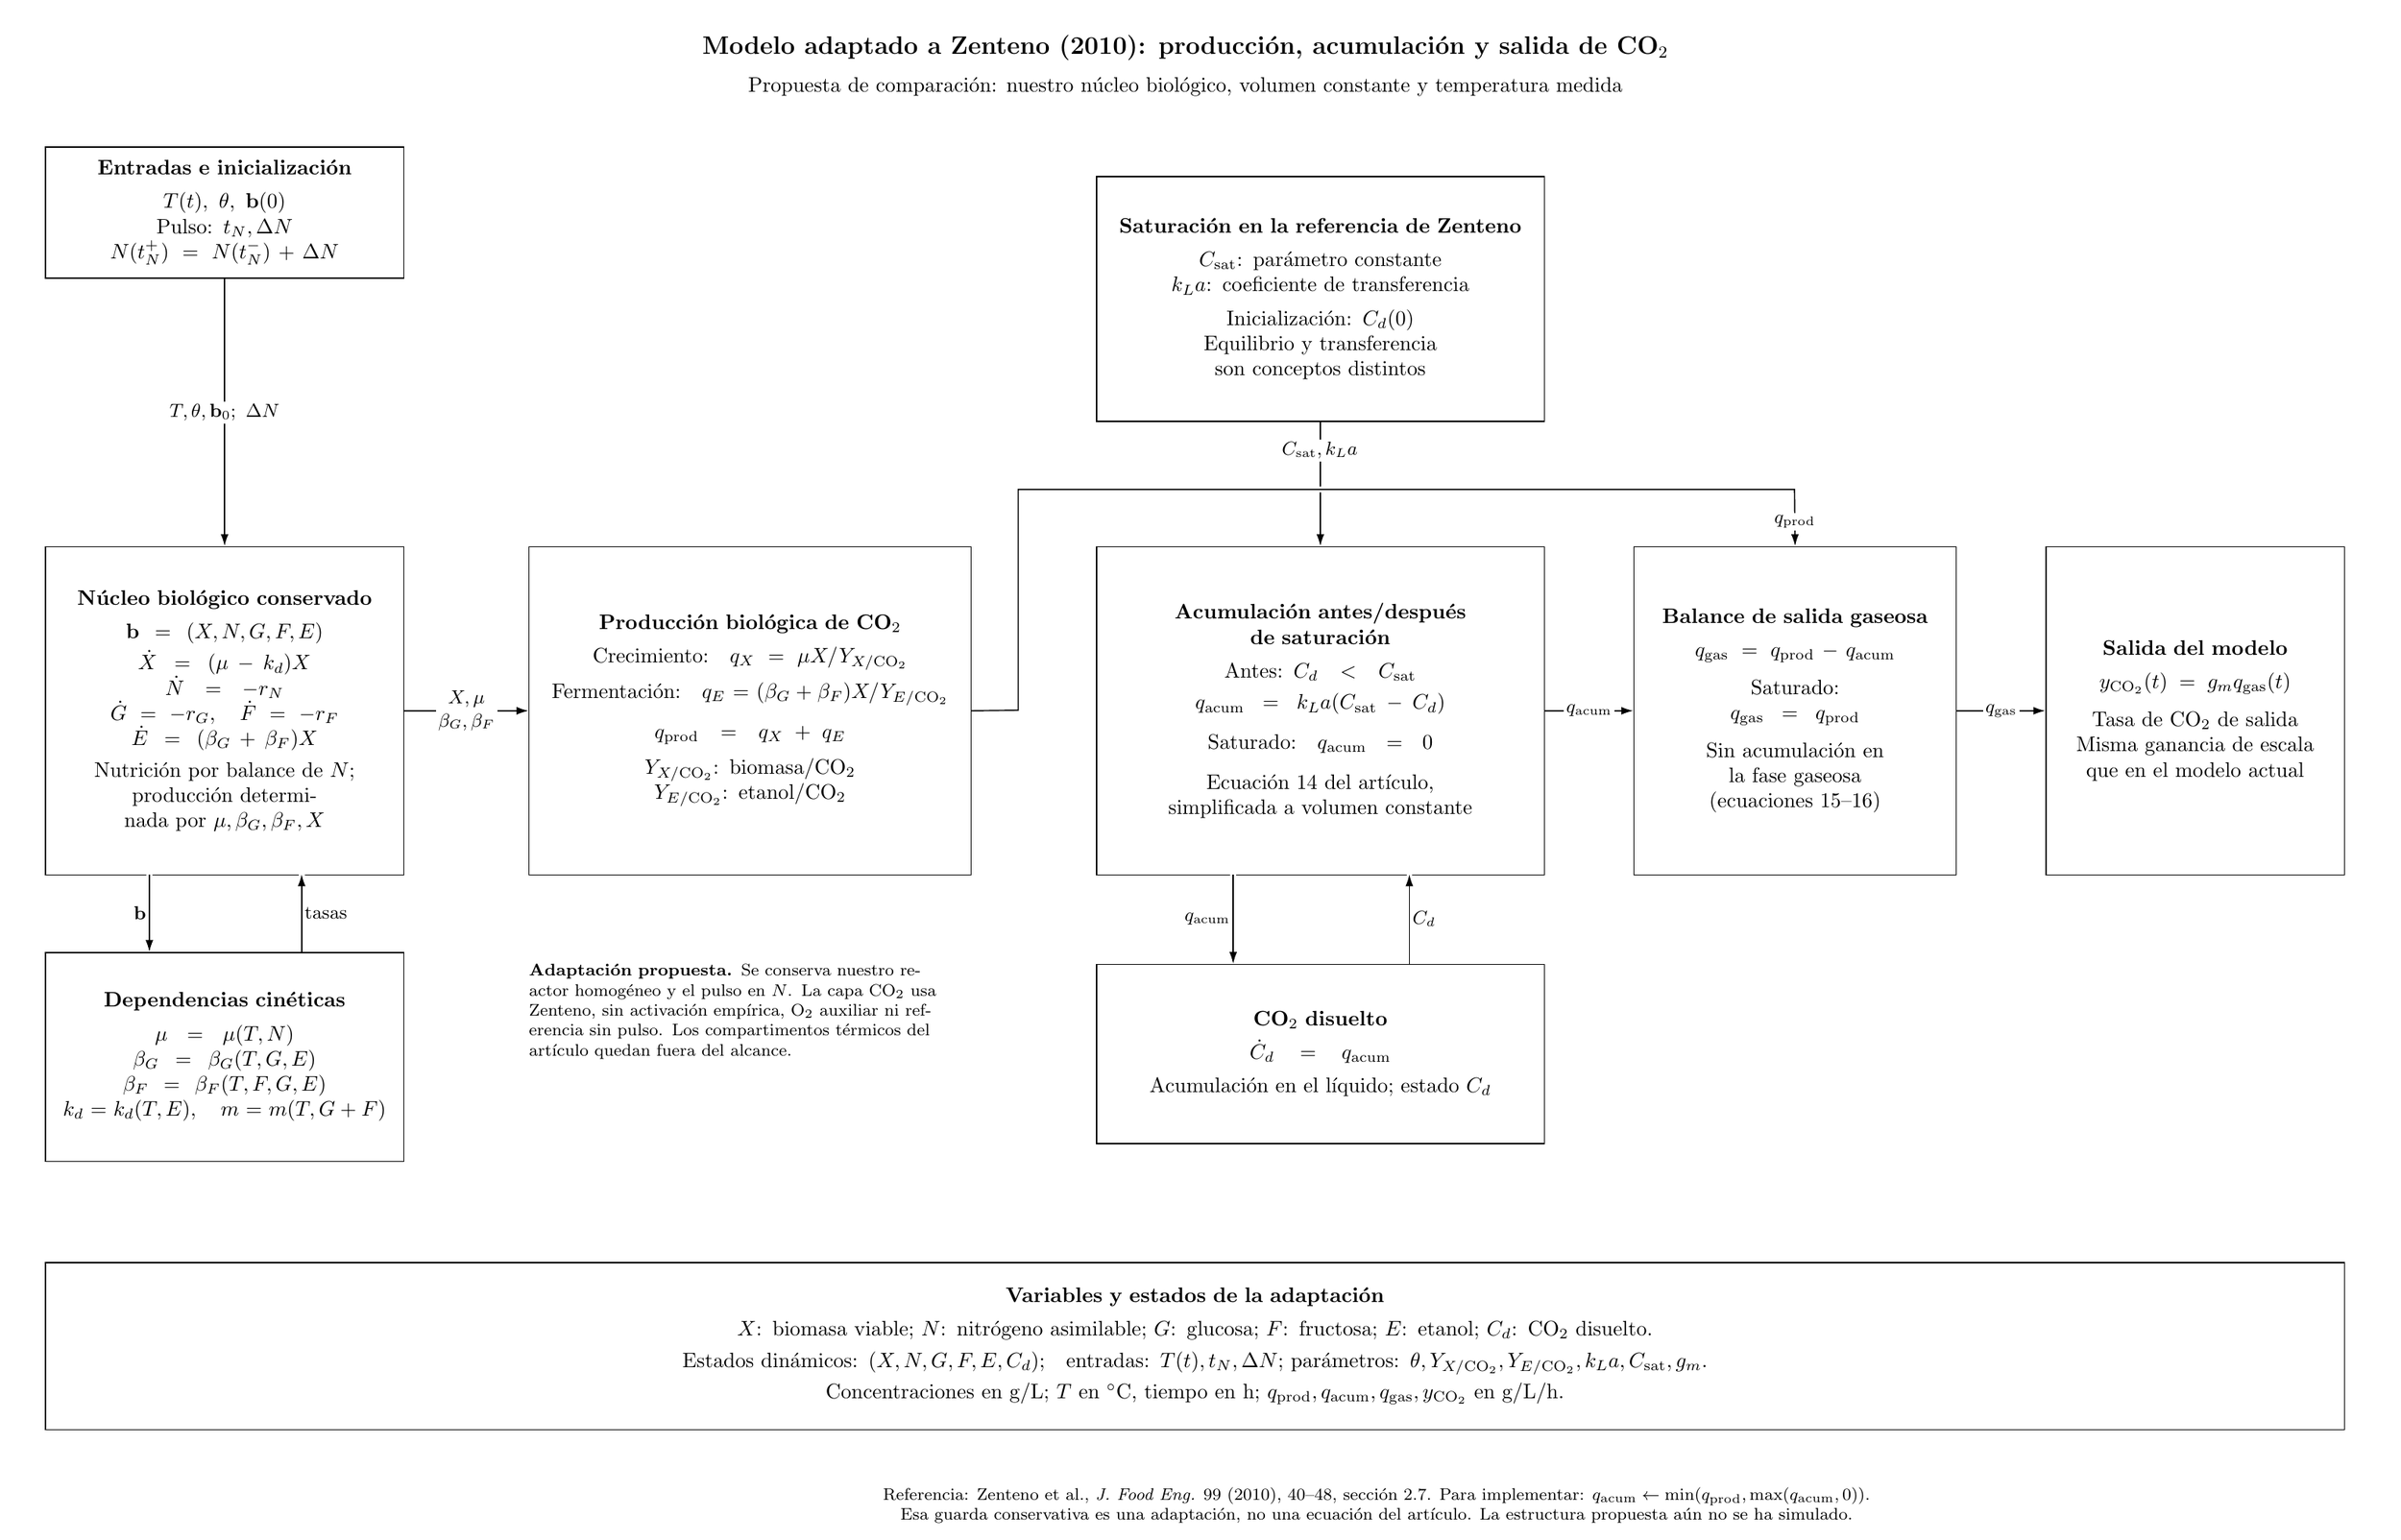
\begin{tikzpicture}[x=1cm,y=1cm,font=\normalsize,line width=.55pt]
\useasboundingbox (0,0) rectangle (39.5,25.1);
\node[font=\large\bfseries] at (19.5,24.65)
  {Modelo adaptado a Zenteno (2010): producción, acumulación y salida de CO\(_2\)};
\node at (19.5,24.0)
  {Propuesta de comparación: nuestro núcleo biológico, volumen constante y temperatura medida};

\block{inputs}{0.4}{23.0}{6.0}{2.2}{Entradas e inicialización}{%
  \(T(t),\ \theta,\ \bb(0)\)\\
  Pulso: \(t_N,\Delta N\)\\
  \(N(t_N^+)=N(t_N^-)+\Delta N\)}
\block{bio}{0.4}{16.3}{6.0}{5.5}{Núcleo biológico conservado}{%
  \(\bb=(X,N,G,F,E)\)\\[3pt]
  \(\dot X=(\mu-k_d)X\)\\
  \(\dot N=-r_N\)\\
  \(\dot G=-r_G,\quad\dot F=-r_F\)\\
  \(\dot E=(\beta_G+\beta_F)X\)\\[3pt]
  Nutrición por balance de \(N\);\\
  producción determinada por \(\mu,\beta_G,\beta_F,X\)}
\block{rates}{0.4}{9.5}{6.0}{3.5}{Dependencias cinéticas}{%
  \(\mu=\mu(T,N)\)\\
  \(\beta_G=\beta_G(T,G,E)\)\\
  \(\beta_F=\beta_F(T,F,G,E)\)\\
  \(k_d=k_d(T,E),\quad m=m(T,G+F)\)}
\block{prod}{8.5}{16.3}{7.4}{5.5}{Producción biológica de CO\(_2\)}{%
  Crecimiento:\quad \(q_X=\mu X/Y_{X/\mathrm{CO_2}}\)\\[5pt]
  Fermentación:\quad \(q_E=(\beta_G+\beta_F)X/Y_{E/\mathrm{CO_2}}\)\\[7pt]
  \(q_{\mathrm{prod}}=q_X+q_E\)\\[5pt]
  \(Y_{X/\mathrm{CO_2}}\): biomasa/CO\(_2\)\\
  \(Y_{E/\mathrm{CO_2}}\): etanol/CO\(_2\)}
\block{sat}{18.0}{22.5}{7.5}{4.1}{Saturación en la referencia de Zenteno}{%
  \(C_{\mathrm{sat}}\): parámetro constante\\
  \(k_La\): coeficiente de transferencia\\[4pt]
  Inicialización: \(C_d(0)\)\\
  Equilibrio y transferencia\\son conceptos distintos}
\block{accum}{18.0}{16.3}{7.5}{5.5}{Acumulación antes/después de saturación}{%
  Antes: \(C_d<C_{\mathrm{sat}}\)\\[3pt]
  \(q_{\mathrm{acum}}=k_La(C_{\mathrm{sat}}-C_d)\)\\[7pt]
  Saturado:\quad \(q_{\mathrm{acum}}=0\)\\[7pt]
  Ecuación 14 del artículo,\\simplificada a volumen constante}
\block{inventory}{18.0}{9.3}{7.5}{3.0}{CO\(_2\) disuelto}{%
  \(\dot C_d=q_{\mathrm{acum}}\)\\[4pt]
  Acumulación en el líquido; estado \(C_d\)}
\block{gas}{27.0}{16.3}{5.4}{5.5}{Balance de salida gaseosa}{%
  \(q_{\mathrm{gas}}=q_{\mathrm{prod}}-q_{\mathrm{acum}}\)\\[6pt]
  Saturado:\\
  \(q_{\mathrm{gas}}=q_{\mathrm{prod}}\)\\[6pt]
  Sin acumulación en\\la fase gaseosa\\
  (ecuaciones 15--16)}
\block{obs}{33.9}{16.3}{5.0}{5.5}{Salida del modelo}{%
  \(y_{\mathrm{CO_2}}(t)=g_mq_{\mathrm{gas}}(t)\)\\[6pt]
  Tasa de CO\(_2\) de salida\\
  Misma ganancia de escala\\que en el modelo actual}
\block{variables}{0.4}{4.3}{38.5}{2.8}{Variables y estados de la adaptación}{%
  \(X\): biomasa viable; \(N\): nitrógeno asimilable; \(G\): glucosa; \(F\): fructosa;
  \(E\): etanol; \(C_d\): CO\(_2\) disuelto.\\[3pt]
  Estados dinámicos: \((X,N,G,F,E,C_d)\);\quad entradas: \(T(t),t_N,\Delta N\);
  parámetros: \(\theta,Y_{X/\mathrm{CO_2}},Y_{E/\mathrm{CO_2}},k_La,C_{\mathrm{sat}},g_m\).\\[3pt]
  Concentraciones en g/L; \(T\) en \(^{\circ}\mathrm C\), tiempo en h;
  \(q_{\mathrm{prod}},q_{\mathrm{acum}},q_{\mathrm{gas}},y_{\mathrm{CO_2}}\) en g/L/h.}

\draw[flow] (inputs.south) -- (bio.north) node[midway,signal] {\(T,\theta,\bb_0;\ \Delta N\)};
\draw[flow] (bio.east) -- (prod.west) node[midway,signal] {\(X,\mu\)\\\(\beta_G,\beta_F\)};
\draw[flow] (sat.south) -- (accum.north);
\draw[flow] (prod.east) -- (16.7,13.55) -- (16.7,17.25) -- (29.7,17.25) -- (gas.north)
  node[pos=.57,signal] {\(q_{\mathrm{prod}}\)};
\node[signal] at (21.75,17.9) {\(C_{\mathrm{sat}},k_La\)};
\draw[flow] (accum.east) -- (gas.west) node[midway,signal] {\(q_{\mathrm{acum}}\)};
\draw[flow] (gas.east) -- (obs.west) node[midway,signal] {\(q_{\mathrm{gas}}\)};
\draw[flow] (20.3,10.8) -- (20.3,9.3) node[midway,signal,left] {\(q_{\mathrm{acum}}\)};
\draw[flow] (23.25,9.3) -- (23.25,10.8) node[midway,signal,right] {\(C_d\)};
\draw[flow] (2.15,10.8) -- (2.15,9.5) node[midway,signal,left] {\(\bb\)};
\draw[flow] (4.7,9.5) -- (4.7,10.8) node[midway,signal,right] {tasas};
\node[anchor=north west,align=left,text width=7.0cm,font=\footnotesize,fill=white,inner sep=0pt]
  at (8.5,9.3)
  {\textbf{Adaptación propuesta.} Se conserva nuestro reactor homogéneo y el pulso en \(N\).
   La capa CO\(_2\) usa Zenteno, sin activación empírica, O\(_2\) auxiliar ni referencia sin pulso.
   Los compartimentos térmicos del artículo quedan fuera del alcance.};
\node[anchor=north,align=center,font=\footnotesize] at (22.7,.65)
  {Referencia: Zenteno et al., \emph{J. Food Eng.} 99 (2010), 40--48, sección 2.7.
   Para implementar: \(q_{\mathrm{acum}}\leftarrow\min(q_{\mathrm{prod}},\max(q_{\mathrm{acum}},0))\).\\
   Esa guarda conservativa es una adaptación, no una ecuación del artículo. La estructura propuesta aún no se ha simulado.};
\end{tikzpicture}
\end{center}
\end{document}
